\documentclass{article}

\usepackage{graphicx}
\usepackage{tikz}
\usepackage{tikzsymbols}
\usetikzlibrary{calc,patterns,shapes.geometric}
\pagestyle{empty}
\usepackage[margin=0pt]{geometry}
\geometry{papersize={14in,12in}}

\def\centerarc[#1](#2)(#3:#4:#5){\draw[#1] ($(#2)+({#5*cos(#3)},{#5*sin(#3)})$) arc (#3:#4:#5);}

\begin{document}
	\begin{figure}
		\centering
		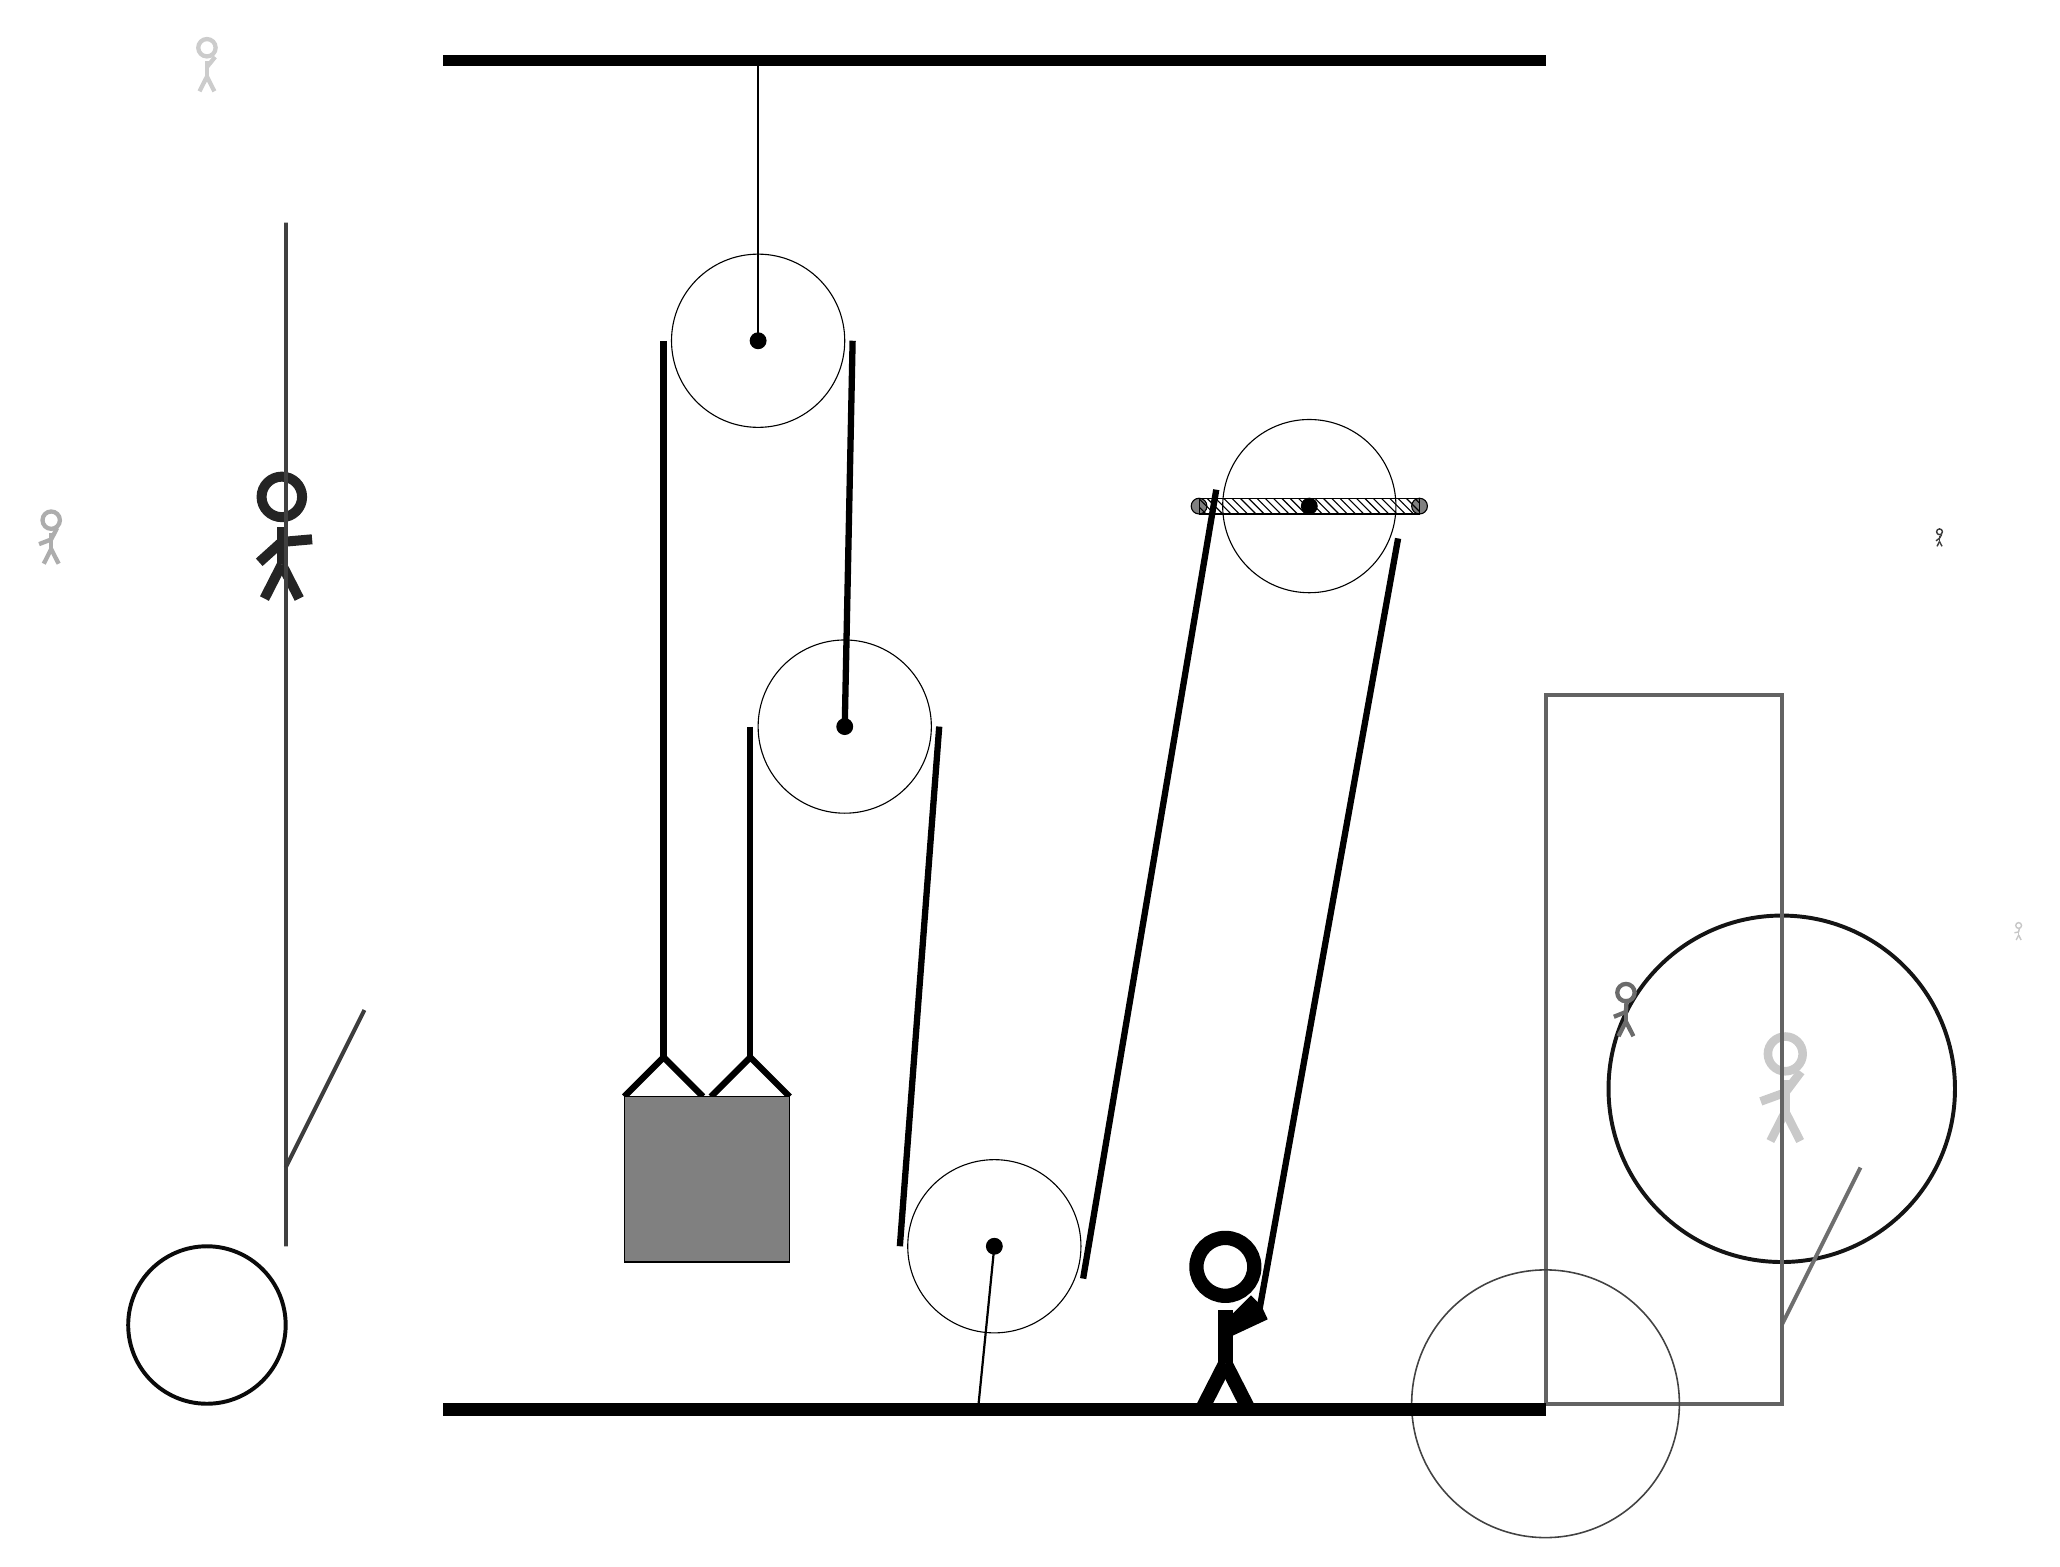
\begin{tikzpicture}
			%%%%% START %%%%%
			
			\draw[fill=black] (-2, 14) rectangle (12, 14.125);
			
			\node[line width=0.2mm, color=black!86] at (-4, 8) {\Strichmaxerl[7][42][5]};
			
			\node[line width=0.7mm, color=black!77] at (17, 8) {\Strichmaxerl[1][37][60]};
			\node[line width=0.4mm, color=black!32] at (-7, 8) {\Strichmaxerl[3][21][63]};
			\node[line width=0.6mm, color=black!21] at (15, 1) {\Strichmaxerl[6][20][53]};
			
			\draw[line width=0.5mm, color=black!75] (-4, 12) rectangle (-4, -1);
			\draw [line width=0.5mm, color=black!92](15, 1) circle (2.2);
			\draw[line width=0.5mm, color=black!76](-3, 2) -- (-4, 0);
			\draw [line width=0.6mm, color=black!40](17, 0) circle (0.0);
			\draw [line width=0.5mm, color=black!96](-5, -2) circle (1.0);
			\node[line width=0.7mm, color=black!20] at (-5, 14) {\Strichmaxerl[3][90][51]};
			\draw[line width=0.5mm, color=black!57](16, 0) -- (15, -2);
			\node[line width=0.4mm, color=black!58] at (13, 2) {\Strichmaxerl[3][22][87]};
			\node[line width=0.5mm, color=black!22] at (18, 3) {\Strichmaxerl[1][11][78]};
			
			\draw[line width=0.5mm, color=black!61] (12, 6) rectangle (15, -3);
			\draw [line width=0.2mm, color=black!74](12, -3) circle (1.7);
			
			\draw (2, 10.5) circle (1.1);
			\draw[fill=black] (2, 10.5) circle (0.1);
			\draw[thick] (2, 10.5) -- (2, 14);
			
			\draw (3.1, 5.6) circle (1.1);
			\draw[fill=black] (3.1, 5.6) circle (0.1);
			
			\draw (5, -1) circle (1.1);
			\draw[fill=black] (5, -1) circle (0.1);
			\draw[thick] (5, -1) -- (4.8, -3);
			
			\draw (9, 8.4) circle (1.1);
			\draw[fill=black] (9, 8.4) circle (0.1);
			\draw[fill=black!50] (7.6, 8.4) circle (0.1);
			\draw[fill=black!50] (10.4, 8.4) circle (0.1);
			\draw[pattern=north west lines, pattern color=black] (7.6, 8.5) rectangle (10.4, 8.3);
			
			\draw[line width = 0.8mm]  (0.3, 0.9) -- (0.8, 1.4) -- (1.3, 0.9);
			\draw[line width = 0.8mm]  (1.4, 0.9) -- (1.9, 1.4) -- (2.4, 0.9);
			\draw[fill=black!50] (0.3, 0.9) rectangle (2.4, -1.2);
			
			\draw[line width = 0.8mm] (0.8, 10.5) -- (0.8, 1.4);
			\centerarc[line width = 0.8mm](2, 10.5)(0:180:1.2000000000000002);
			\draw[line width = 0.8mm] (3.2, 10.5) -- (3.1, 5.6);
			\draw[line width = 0.8mm] (1.9, 5.6) -- (1.9, 1.4);
			\centerarc[line width = 0.8mm](3.1, 5.6)(0:180:1.2000000000000002);
			\draw[line width = 0.8mm] (4.3, 5.6) -- (3.8, -1);
			\centerarc[line width = 0.8mm](5, -1)(180:340:1.2000000000000002);
			\draw[line width=0.8mm](6.1276, -1.4104) -- (7.8182, 8.6083);
			\centerarc[line width = 0.8mm](9, 8.4)(-20:170:1.2000000000000002);
			\draw[line width=0.8mm](10.1276, 7.9896) --  (8.35, -1.9);
			
			\node at (8, -2) {\Strichmaxerl[10][225][25]};
			
			\draw[fill=black] (-2, -3) rectangle (12, -3.15);
			
			%%%%% END %%%%%
		\end{tikzpicture}
	\end{figure}	
\end{document}